


\section{DOI Data Collection is non-trivial}
\label{sec:DOINonTrivial}
Many eye-tracking related studies generate visual stimuli using computer programs coded by visualization researchers. In such cases, since the structure and layout of the visual content in the stimuli is accessible at runtime, we can relate gaze positions supplied on the fly by an eye-tracker to the visual content of such visualizations.

For example, in Figure~\ref{fig:Miserables}, a network diagram depicts the characters from the novel Les Miserables. Links between two characters are present if they co-occurred in the same chapter. The colors indicate different clusters of characters. The visualization has interactions such as dragging nodes (i.e. rectangles). Moreover, users can input a `compactness' value to change the layout of the visualization. The lower value of compactness indicates a compact arrangement of the network. Figure~\ref{fig:MiserablesCompactness} shows the same visualization with four different compactness values. 


\begin{figure}[htb]
  \centering
  \includegraphics[width=0.99\linewidth]{images/Miserables.eps}
  \caption{An interactive network visualization, depicting characters from Les Miserables. Each rectangle node represents a character and links represent character co-occurrence in the same chapter. Different colors represent different clusters of characters. Interaction such as dragging nodes is available for this visualization.}
    \label{fig:Miserables}
\end{figure}

\begin{figure}[htb]
  \centering
  \includegraphics[width=0.99\linewidth]{images/MiserablesCompactness.eps}
  \caption{Different layouts of Les Miserables visualization when the compactness is changed.}
    \label{fig:MiserablesCompactness}
\end{figure}

Figure~\ref{fig:MiserablesSimple} is a smaller version of the original network diagram with the major characters only. This figure also depicts collected gaze points from a user looking at Fantine and Cosette. It is evident that we can match the positions of these gaze samples to the two rectangles closest to them (i.e. the visual content). Hence, we label this eye-tracking analysis as being in `visualization space' (i.e., relating gazes to visual objects shown on the screen) rather than 'image space' (i.e., relating gazes to pixels in a stimulus).

\begin{figure}[htb]
  \centering
  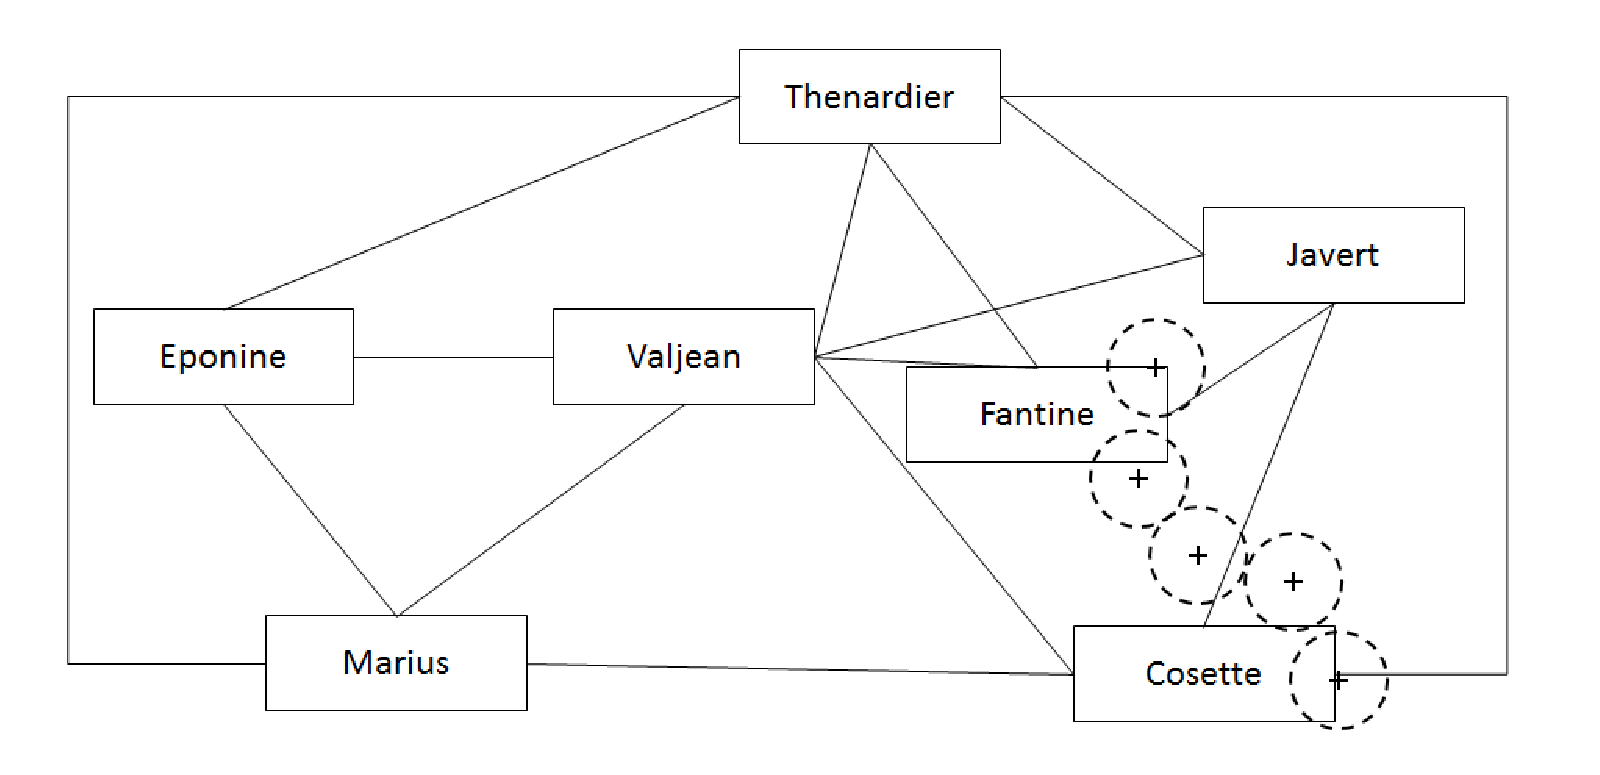
\includegraphics[width=0.99\linewidth]{images/MiserablesSimple.eps}
  \caption{: A network diagram with major characters of Les Miserables. The dashed circles represent a user's gazes. Here, most gaze points are adjacent to Fantine and Cosette. }
    \label{fig:MiserablesSimple}
\end{figure}

Moreover, the visual objects are shown in the Les Miserables visualization stand for actual data: the characters in the novel. So, mapping gazes to the visual objects let us in turn map the user's interest to data elements, such as Fantine and Cosette. Moreover, by looking at the properties of the data that users are viewing, we can relate visual interest to semantic data subsets or perspectives. For example, Fantine and Cosette are both female characters and, based solely on the few gaze samples depicted in our example. We could conclude that the user is viewing female characters. In other words, we can track the user's interest in data subsets defined based on gender. Similar data subsets could be identified based on central or secondary characters, positive or negative characters, etc. We call this eye-tracking data analysis in ``data space'' or data of interest (DOI) analysis.

We hypothesize that this is a compelling alternative to traditional analysis methods, primarily AOI (area of interest) analyses. Using conventional AOI-based approaches, analyzers would be required to define AOIs over already rendered 2D stimuli. In our example, and most real-life visualizations, this would be time-consuming because of the many visual objects displayed on the screen. Moreover, the 2D layout of the visualization may change in response to user interactions (e.g., users move node), in which case the AOI annotations would need to change. Moreover, AOIs are not annotated by any attributes so defining AOIs on characters wouldn't implicitly mean that we could also track other data subsets such as based on gender.  

However, as described in Chapter~\ref{chap:Intro}, mapping gazes to individual data objects is bound to be imprecise since eye-trackers produce noisy, low-resolution data. Figure ~\ref{fig:MiserablesGaze} illustrates this. We can use the na\"{i}ve approach of mapping gazes to the nearest visual object. Using this approach, we can confidently map $g_1, g_2$ to Fontaine, and $g_4, g5$ to Cosette. However, it's less clear what we should do about $g_3$ since it's squarely between the two nodes. 

\begin{figure}[htb]
  \centering
  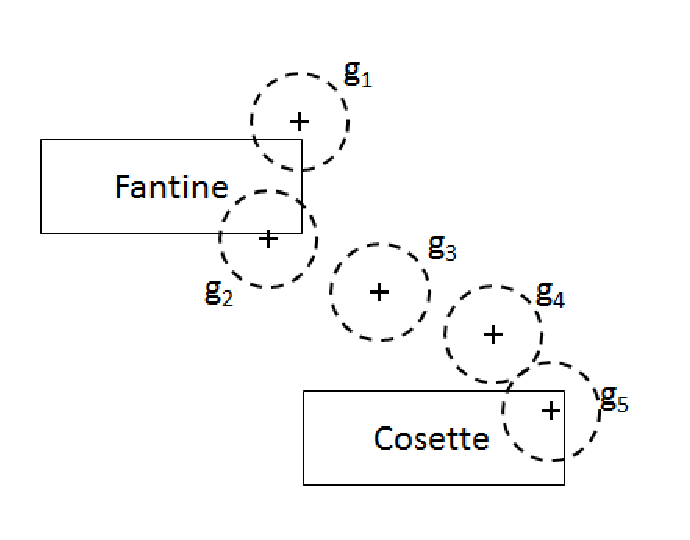
\includegraphics[width=0.5\linewidth]{images/MiserablesGaze.eps}
  \caption{: Using proximity alone to map gazes to visual objects. We have 2 rectangles Fontaine and Cosette, and five gazes $g_1, g_2, g_3, g_4, g_5$. Each gaze is to be mapped to either Fontaine or Cosette. $g_1, g_2$ maps to Fontaine and $g_4$ map to Cosette. However, $g_3$ cannot be mapped directly to neither Fontaine nor Cosette. }
    \label{fig:MiserablesGaze}
\end{figure}